%%%%%%
%
% $Autor: Sudeshna Nanda $
% $Datum: 2024-10-18 $
% $Pfad: ML23-06-Magic-Wand-with-an-Arduino-Nano-33-BLE-sense/manual/Contents/en/Overview.tex $
% $Version: 1 $
%
%%%%%%


\chapter{Overview}

\section{What's in the box?}

Make sure the following items are included with your box. If any items are missing, contact your dealer at once.

\begin{enumerate}
	\item Magic Wand
	\item Data Transformation and Charging Micro-USB Cable
	\item User Manual
\end{enumerate}

\begin{figure}[h]\centering
	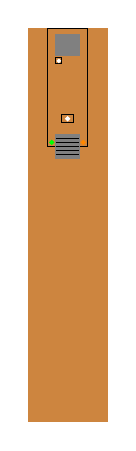
\begin{tikzpicture}[scale=0.5]

			% Define colors
			\definecolor{woodcolor}{RGB}{205,133,63} % A color for the wooden dowel
			\definecolor{boardcolor}{RGB}{30,30,30}  % A color for the microcontroller board
			\definecolor{sharporange}{RGB}{255,135,0}
			
			\filldraw[woodcolor] (-1,4.5) rectangle (1,-5.5);
			\draw  (-0.5,4.5) rectangle (0.5,1.5);
			\filldraw[gray]  (-0.3,1.8) rectangle (0.3,1.2);
			\filldraw[green]  (-0.4,1.6) node (v2) {} circle [radius=0.05];
			\filldraw[sharporange]  (0.4,1.6) circle [radius=0.05];
			\filldraw[gray]  (-0.3,4.35) rectangle (0.3,3.8);
			\draw  (-0.3,3.75) rectangle (-0.15,3.6);
			\draw (-0.3,1.7) -- (0.3,1.7);
			\draw (-0.3,1.6) -- (0.3,1.6);
			\draw (-0.3,1.5) -- (0.3,1.5);
			\draw (-0.3,1.4) -- (0.3,1.4);
			\draw (-0.3,1.3) -- (0.3,1.3);
			\draw  (0.15,2.1) rectangle (-0.15,2.3);
			\filldraw[white]  (0,2.2) circle[radius=0.05];
			\filldraw[white]  (-0.22,3.67) circle[radius=0.04];
			%\node (v1) at (-2.5,1.5) {Power Led};
			%\draw (v1) -- (v2);
			
	\end{tikzpicture}
	\caption{\textbf{Magic Wand}}
\end{figure}

\begin{figure}[h]\centering
	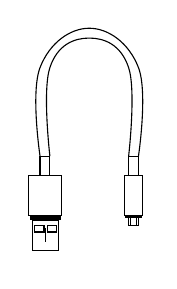
\begin{tikzpicture}[scale=0.25]
		
		\draw  (-1.5,-0.5) node (v3) {} rectangle (-1,-1.5);
		\draw  (-2.1,-1.5) rectangle (-0.4,-3.5);
		\filldraw (-2,-3.5) rectangle (-0.45,-3.7);
		\draw  (-1.9,-3.75) rectangle (-0.55,-5.3);
		\node (v2) at (-1.2,-3.65) {};
		\node (v1) at (-1.2,-5.35) {};
		\draw  (v1) edge (v2);
		\draw  (-1.8,-4) rectangle (-1.3,-4.35);
		\draw  (-1.1,-4) rectangle (-0.65,-4.35);
		\draw  plot[smooth, tension=.7] coordinates {(v3) (-1.5,4) (1,6) (3.5,4) (3.5,-0.5)};
		\draw  (3,-0.5) node (v4) {} rectangle (3.5,-1.5);
		\draw  plot[smooth, tension=.7] coordinates {(-1,-0.5) (-1,4) (1,5.5) (3,4) (v4)};
		\draw  (2.8,-1.5) rectangle (3.7,-3.5);
		\filldraw  (2.85,-3.5) rectangle (3.65,-3.6);
		\draw  (3,-3.5) rectangle (3.5,-4);
		\draw (3.1,-4) -- (3.1,-3.5);
		\draw (3.4,-4) -- (3.4,-3.5);
	\end{tikzpicture}
	\caption{\textbf{Micro USB Cable}}
\end{figure}

\begin{figure}[h]\centering
	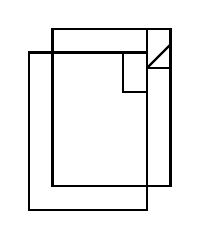
\begin{tikzpicture}[scale=1]
		% First rectangle with a folded corner
		\draw[thick] (0,0) rectangle (1.5,2);
		\draw[thick] (1.5,1.5) -- (1.2,1.5) -- (1.2,2);
		
		% Second rectangle partially behind the first one
		\draw[thick] (0.3,0.3) rectangle (1.8,2.3);
		
		% Folded corner on the second rectangle
		\draw[thick] (1.8,1.8) -- (1.5,1.8) -- (1.5,2.3);
		
		% The line indicating the fold
		\draw[thick] (1.5,1.8) -- (1.8,2.1);
		
		% Optional shading for the folded part to give depth (requires tikz library)
		%\fill[gray!30] (1.5,1.8) -- (1.8,2.1) -- (1.8,1.8) -- cycle;
		%\fill[gray!30] (1.2,1.5) -- (1.5,1.8) -- (1.5,1.5) -- cycle;
	\end{tikzpicture}
	\caption{\textbf{User Manual}}
\end{figure}

\pagebreak

\begin{itemize}
	\item The items’ colours and shapes may vary depending on the models.
	\item Please check for any accessories hidden behind or in the packing materials when opening the box.
\end{itemize}

\textbf{Warning:} The board can be damaged from direct pressure when handled incorrectly. We recommend toughing the board at the edges. 

\bigskip

\section{Overview of Magic Wand}

\subsection{Top View of Magic Wand}

\begin{figure}[h]\centering
	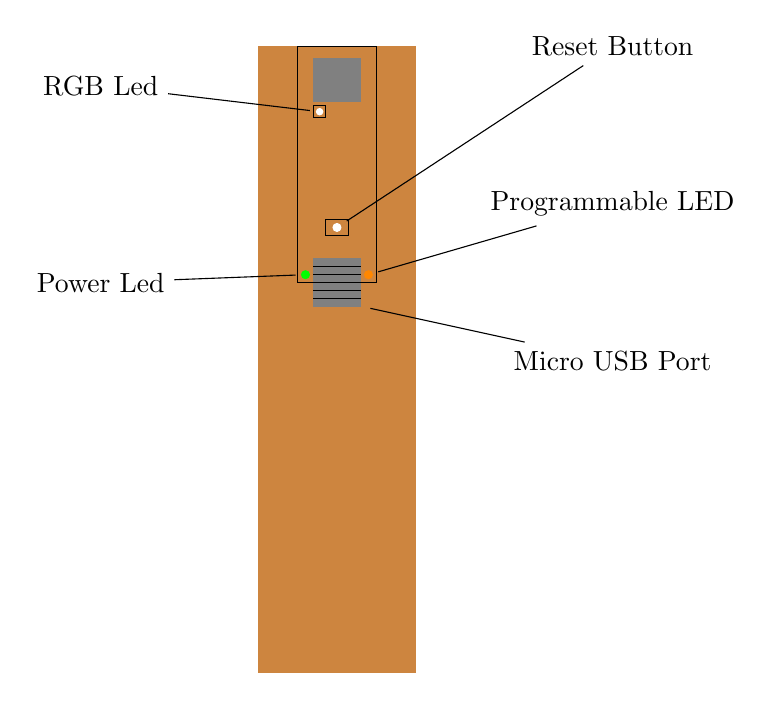
\begin{tikzpicture}
		% Define colors
		\definecolor{woodcolor}{RGB}{205,133,63} % A color for the wooden dowel
		\definecolor{boardcolor}{RGB}{30,30,30}  % A color for the microcontroller board
		\definecolor{sharporange}{RGB}{255,135,0}
		
		\filldraw[woodcolor] (-1,4.5) rectangle (1,-3.45);
		\draw  (-0.5,4.5) rectangle (0.5,1.5);
		\filldraw[gray]  (-0.3,1.8) rectangle (0.3,1.2) node (v5) {};
		\filldraw[green]  (-0.4,1.6) node (v2) {} circle [radius=0.05];
		\filldraw[sharporange]  (0.4,1.6) node (v9) {} circle [radius=0.05];
		\filldraw[gray]  (-0.3,4.35) rectangle (0.3,3.8);
		\draw  (-0.3,3.75) rectangle (-0.15,3.6);
		\draw (-0.3,1.7) -- (0.3,1.7);
		\draw (-0.3,1.6) -- (0.3,1.6);
		\draw (-0.3,1.5) -- (0.3,1.5);
		\draw (-0.3,1.4) -- (0.3,1.4);
		\draw (-0.3,1.3) -- (0.3,1.3);
		\draw  (0.15,2.1) rectangle (-0.15,2.3);
		\filldraw[white]  (0,2.2) node (v7) {} circle[radius=0.05];
		\filldraw[white]  (-0.22,3.67) node (v4) {} circle[radius=0.04];
		\node (v1) at (-3,1.5) {Power Led};
		\draw (v1) -- (v2);
		\node (v3) at (-3,4) {RGB Led};
		\draw  (v3) edge (v4);
		
		\node (v6) at (3.5,0.5) {Micro USB Port};
		\draw  (v5) edge (v6);
		\node (v8) at (3.5,4.5) {Reset Button};
		\draw  (v7) edge (v8);
		\node (v10) at (3.5,2.5) {Programmable LED};
		\draw  (v9) edge (v10);
	\end{tikzpicture}
	\caption{\textbf{Magic Wand Top View}}
\end{figure}

\pagebreak

\subsection{Front View of Magic Wand}

\begin{figure}[h]\centering
	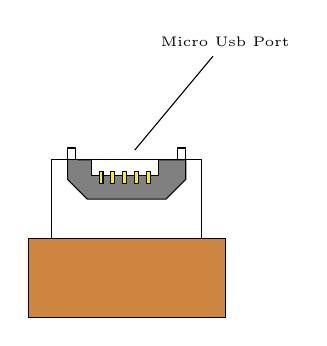
\begin{tikzpicture}
		\definecolor{woodcolor}{RGB}{205,133,63}
		\filldraw[fill=woodcolor, draw=black]  (-1,0) rectangle (1.5,-1);
		\draw  (-0.7,1) rectangle (1.2,0);
		
		\filldraw[fill=gray] (-0.5,1) node (v1) {} -- (-0.5,0.75) -- (-0.25,0.5) -- (0,0.5) -- (0.5,0.5) -- (0.75,0.5) -- (1,0.75) -- (1,1) -- (0.25,1) node (v2) {} -- (v1);
		\filldraw[fill=white, draw=black]  (-0.2,1) rectangle (0.65,0.8);
		\filldraw[fill=yellow,  draw=black]  (-0.1,0.85) rectangle (-0.05,0.7);
		\filldraw[fill=yellow,  draw=black] (0.1,0.85) rectangle (0.05,0.7);
		\filldraw[fill=yellow,  draw=black]  (0.2,0.85) rectangle (0.25,0.7);
		\filldraw[fill=yellow,  draw=black]  (0.35,0.85) rectangle (0.4,0.7);
		\filldraw[fill=yellow,  draw=black]  (0.5,0.85) rectangle (0.55,0.7);
		\draw  (-0.5,1.15) rectangle (-0.4,1);
		\draw  (0.9,1.15) rectangle (1,1);
		\draw (0,1);
		\node[font=\tiny] (v3) at (1.5,2.5) {Micro Usb Port};
		\draw  (v2) edge (v3);
		
	\end{tikzpicture}
	\caption{\textbf{Magic Wand Front View}}
\end{figure}

\begin{enumerate}
	\item \textbf{Power LED} - See "Switching On"\ref{switching on}
	\item \textbf{Reset Button} - See "Reset Magic Wand"\ref{Reset Magic Wand}
	\item \textbf{RGB LED} - See "Motion Movement"\ref{Motion Movement}
	\item \textbf{Micro-USB Port} - Connect the main micro USB cable here. See "Switching On" \ref{switching on}
	\item \textbf{Placing the unit}
	\begin{itemize}
		\item The Magic Wand should never be placed near a fire or other source of heat.
		\item Avoid placing any other part or object on top of the board since this could harm the sensor and make it unable to detect motion correctly.
		\item When connecting the cable, be sure to only touch the board's edge to avoid contact with any conductive areas.
	\end{itemize}
\end{enumerate}


